\documentclass[aip,apl,reprint]{revtex4-1}
\usepackage{graphicx}
\usepackage{bm}
\usepackage{color}

\begin{document}

\title{Propagation length of mid-infrared surface plasmon polaritons \color{red}on gold: impact of morphology change by thermal annealing\color{black}}
\author{Nobuyoshi Hiramatsu}
%\author{N. Hiramatsu}
\altaffiliation[Also at ]{Department of Applied Physics, Faculty of Engineering, the University of Tokyo, 7-3-1 Hongo, Bunkyo-ku, Tokyo 113-8656, Japan}
\affiliation{Institute of Industrial Science, the University of Tokyo, 4-6-1 Komaba, Meguro-ku, Tokyo 153-8505, Japan}
\author{Fumiya Kusa}
%\author{F. Kusa}
\affiliation{Institute of Industrial Science, the University of Tokyo, 4-6-1 Komaba, Meguro-ku, Tokyo 153-8505, Japan}
\author{Akinobu Takegami}
%\author{A. Takegami}
\affiliation{Institute of Industrial Science, the University of Tokyo, 4-6-1 Komaba, Meguro-ku, Tokyo 153-8505, Japan}
\author{Kotaro Imasaka}
%\author{K. Imasaka}
\affiliation{Institute of Industrial Science, the University of Tokyo, 4-6-1 Komaba, Meguro-ku, Tokyo 153-8505, Japan}
\author{Ikki Morichika}
%\author{I. Morichika}
\affiliation{Institute of Industrial Science, the University of Tokyo, 4-6-1 Komaba, Meguro-ku, Tokyo 153-8505, Japan}
\author{Satoshi Ashihara}
%\author{S. Ashihara}
%\thanks{Corresponding author.}
\email{ashihara@iis.u-tokyo.ac.jp}
\affiliation{Institute of Industrial Science, the University of Tokyo, 4-6-1 Komaba, Meguro-ku, Tokyo 153-8505, Japan}

\date{\today}

\begin{abstract}
We \color{red}studied \color{black}propagation length of surface plasmon polaritons (SPPs) at gold/air interface \color{red}in the mid-infrared range. \color{black}We showed that SPPs propagate for a distance \color{red}about or above \color{black}$10\:\mathrm{mm}$ at a wavelength of $10.6\:\mathrm{\mu m}$, in good agreement with the value predicted from the dielectric constant of polycrystalline gold. We \color{red}also \color{black}demonstrated that \color{red}simple treatment of thermal annealing led to noticeable elongation of the SPP propagation length, which was correlated with increased crystallite grain size and decreased surface roughness. \color{black}Quantitative evaluation of the SPP propagation length, \color{red}in correlation with material's morphology, \color{black}is important in designing plasmonic devices and beneficial for deeper understandings on the mechanisms of losses \color{red}which underly \color{black}achievable electric-field enhancements.
\end{abstract}

\maketitle
 
\section{Introduction}
Plasmonics in the mid-infrared (IR) range has gained increasing attention,\cite{Stanley, Law} because of \color{red}possible \color{black}applications to surface-enhanced spectroscopy,\cite{Neubrech, Hoang} chemical/bio sensing,\cite{Cleary2008} thermal radiation control,\cite{Kusunoki} optoelectronic circuit,\cite{Ebbesen, Soref} nonlinear light-matter interactions,\cite{Kusa2015} etc. Surface plasmons (SPs), including surface plasmon polaritons (SPPs) and localized surface plasmons (LSPs), can be excited at mid-IR wavelengths on various materials.\cite{Law} The behaviors of SPs, however, significantly vary according to the material where they are excited.\cite{Law} 

\color{red}SPs on highly-doped semiconductors and graphenes that have plasma frequencies in the mid-IR range \color{black}are closely bound to the material surface, exhibiting wavelength shortening and large Ohmic loss at mid-IR wavelengths. Therefore, these materials are suited for achieving subwavelength confinement. \color{red}SPs on noble metals that have plasma frequencies in the visible range, on the other hand, \color{black}are weakly bound to the material surface, exhibiting subtle wavelength shortening and small Ohmic loss at mid-IR wavelengths. Therefore noble metals are advantageous in applications where any of small loss, long propagation length, and large electric-field enhancement is required.\cite{Law, Kusa2014}
\color{red}Among noble metals, gold is an excellent plasmonic material, because of its high metallic conductivity and superior chemical stability.\cite{Zayats}\color{black}

Propagation length of SPPs is an important physical quantity \color{red}because \color{black}it sets \color{red}available physical size of plasmonic devices in applications like \color{black}sensors and optoelectronic circuits. \color{red}It is also important as \color{black}a direct measure of SPP's losses, which underly the degree of electric-field enhancement \color{red}achievable upon excitations of SPPs and LSPs. \color{black}Electric-field enhancement plays key roles in many plasmonic applications.

In general, \color{red}SPPs decay \color{black}by radiative damping and irradiative damping. Radiative damping occurs by coupling with \color{red}(or scattering into) \color{black}free-propagating light and other SPP states. Irradiative damping originates from scattering of free electrons by electrons, phonons, defects, impurities, crystallite grain boundaries, etc., and is frequently referred to as the Ohmic loss. Both of the radiative and irradiative damping rates depend on microscopic structure of materials. Therefore, evaluation of the SPP propagation length, together with characterization of material morphology, helps us understand the loss mechanisms of SPPs.

\color{red}The early studies of 1970's and 1980's reported propagation length of mid-IR SPPs on polycrystalline metal films of gold,\cite{McMullen, Schlesinger1, Schlesinger2} silver,\cite{Schlesinger1, Schlesinger2} and copper.\cite{Schoenwald, Shiba} The reported values were, however, inconsistent with each other, and it was difficult to get deeper insights since material's morphology was not characterized. Nowadays it is possible to characterize material's morphology by a variety of scanning probe microscopy techniques. In fact, the propagation length of SPPs on gold at visible wavelengths\cite{Kuttge} and dielectric function of gold\cite{Trollmann, Olmon} have been studied in correlation with morphology observed by atomic force microscopy (AFM) in recent publications. There has been, however, no report on the propagation length of mid-IR SPPs on gold, with simultaneous characterization of morphology.\color{black}

\color{red}In this study, we experimentally measured the propagation length of SPPs at gold/air interface at a mid-IR wavelength of $10.6\:\mathrm{\mu m}$ and correlated it with morphology of gold.\color{black} Here we characterized the morphology by AFM, scanning electron microscopy (SEM), and electron backscatter diffraction (EBSD). We showed that the SPPs propagate for a distance about or above $10\:\mathrm{mm}$, in agreement with the value predicted from the dielectric constant of polycrystalline gold. \color{red}Furthermore, \color{black}we demonstrated that the SPP propagation length can be increased by a simple treatment of thermal annealing, accompanied by increased grain size and suppressed surface roughness.
In this study, we designed and utilized surface-relief gratings as input/output couplers. Compared with the prism coupling technique,\cite{Schoenwald, Shiba} the grating coupling technique does not suffer from contamination of collinear radiative components.\cite{Schlesinger1, Schlesinger2} Compared with the edge coupling technique,\cite{Schlesinger1, Schlesinger2} the grating coupling technique provides higher coupling efficiency and the resultant better signal-to-noise ratio. 

\section{Device design and fabrication}
\label{sec:device}
In order to measure the propagation length of SPPs, we designed a series of SPP waveguide devices. Each device consists of an input coupler, an SPP waveguide, and an output coupler.  The input and output couplers are surface relief gratings made of gold. SPPs are  excited at the input coupler from freely-propagating light, propagate along the SPP waveguide, and are re-converted to freely-propagating light at the output coupler, as illustrated in Fig. \ref{fig:device}(a). The input-output power ratio \color{red}should be a product of \color{black}light-SPP coupling efficiency, \color{red}SPP propagation efficiency (or transmittance), \color{black}and SPP-light coupling efficiency. 

Therefore, if the input/output coupling efficiencies are identical among all devices, we can deduce the propagation length (the distance that SPP power falls to $1/e$ of its initial value), by measuring the input-output power ratio for devices with different waveguide lengths.  In the experiments, we assumed that the coupling efficiencies are identical among all devices and measured output optical power for each device, while keeping incident optical power constant. 

Freely-propagating light and SPPs can be coupled to each other by using a grating structure which satisfies the condition\cite{Koev},
\begin{equation}
k_{\mathrm{SPPgr}}=k_0 \sin \theta + \frac{2m\pi}{d},
\label{eq:phase-match}
\end{equation}
where $k_{\mathrm{SPPgr}}$ and $k_0=2\pi/\lambda_0$ are the wavenumbers of SPP at the grating and that of light in free space, respectively, $\lambda_0$ is the wavelength of light in free space, $\theta$ is an incident angle, $d$ is a grating pitch, and $m$ is an integer. Here we note that $k_{\mathrm{SPPgr}}$ is close to the SPP wavenumber on a flat film in the case of shallow gratings.

Grating depth is known to be influential for the light-SPP (SPP-light) coupling efficiency\cite{Koev, Cleary2010}. To find the optimum grating \color{red}depth \color{black}for maximum coupling, we conducted numerical simulations on reflection efficiencies of surface relief gratings made of gold, by the rigorous coupled-wave analysis (RCWA)\cite{Leveque}. 

Here, we assumed that each grating is made of polycrystalline gold, and has a rectangular profile, a pitch of $15\:\mathrm{\mu m}$, and a duty cycle of 0.5. Incident light was assumed to be a plane monochromatic wave at a wavelength of $10.6\:\mathrm{\mu m}$. 
Figure \ref{fig:device}(b) shows the calculated \color{red}energy \color{black}reflection efficiency as a function of incident angle and grating depth. The reflection efficiency reveals a dip at the grating depth \color{red}of \color{black}0.2-1.3 $\mathrm{\mu m}$ and at the incident angle of 17-18 degree. The \color{red}energy \color{black}loss in reflection \color{red}is due to \color{black}conversion from freely-propagating light to SPPs.
Considering the possible beam convergence of the incident light, we chose the grating depth of $0.8\:\mathrm{\mu m}$ for efficient coupling. Our choice is close to the conclusion derived by Cleary et al.\cite{Cleary2010} that the optimum grating depth of a rectangular grating \color{red}was \color{black}10\%-15\% of the wavelength in the mid-IR range.

Physical dimensions of \color{red}our devices \color{black}are presented in Fig.\ref{fig:device}(a).  The SPP waveguides have a common width of $0.5\:\mathrm{mm}$ and varied lengths $L$ of $3, 5, 7, 9,$ and $11\:\mathrm{mm}$. The input (output) coupler is $1\:\mathrm{mm}$ in length and $0.5\:\mathrm{mm}$ ($1.5\:\mathrm{mm}$) in width. Both of the input and output couplers have rectangular profiles with a grating pitch of $15\:\mathrm{\mu m}$ and a duty cycle of 0.5. As will be described below, the waveguides and the gratings were fabricated to have a common hight of $0.8\:\mathrm{\mu m}$ from a gold base layer.

The devices were fabricated by means of electron beam lithography, thermal evaporation, and lift-off process. A gold base layer with a thickness of $200\:\mathrm{nm}$ was thermally evaporated on a silica glass substrate with a 5-nm-thick chromium adhesion layer, after the substrate was cleaned with acetone and ethanol. Then, electron-beam resist (OEBR-CAP112PM, Tokyo Ohka Kogyo Co., Ltd) was spin-coated with a thickness of $1700\:\mathrm{nm}$, exposed by electron beam, and developed. Finally, gold with a thickness of $800\:\mathrm{nm}$ was deposited on the developed resist, which was then lifted off by acetone. \color{red}During the evapolation process, the substrate was not heated. We \color{black}maintained the evaporation rate of gold to be $0.4\:\mathrm{nm/s}$, and the pressure inside the vacuum chamber to be less than $4\:\mathrm{mPa}$.

 \begin{figure}
    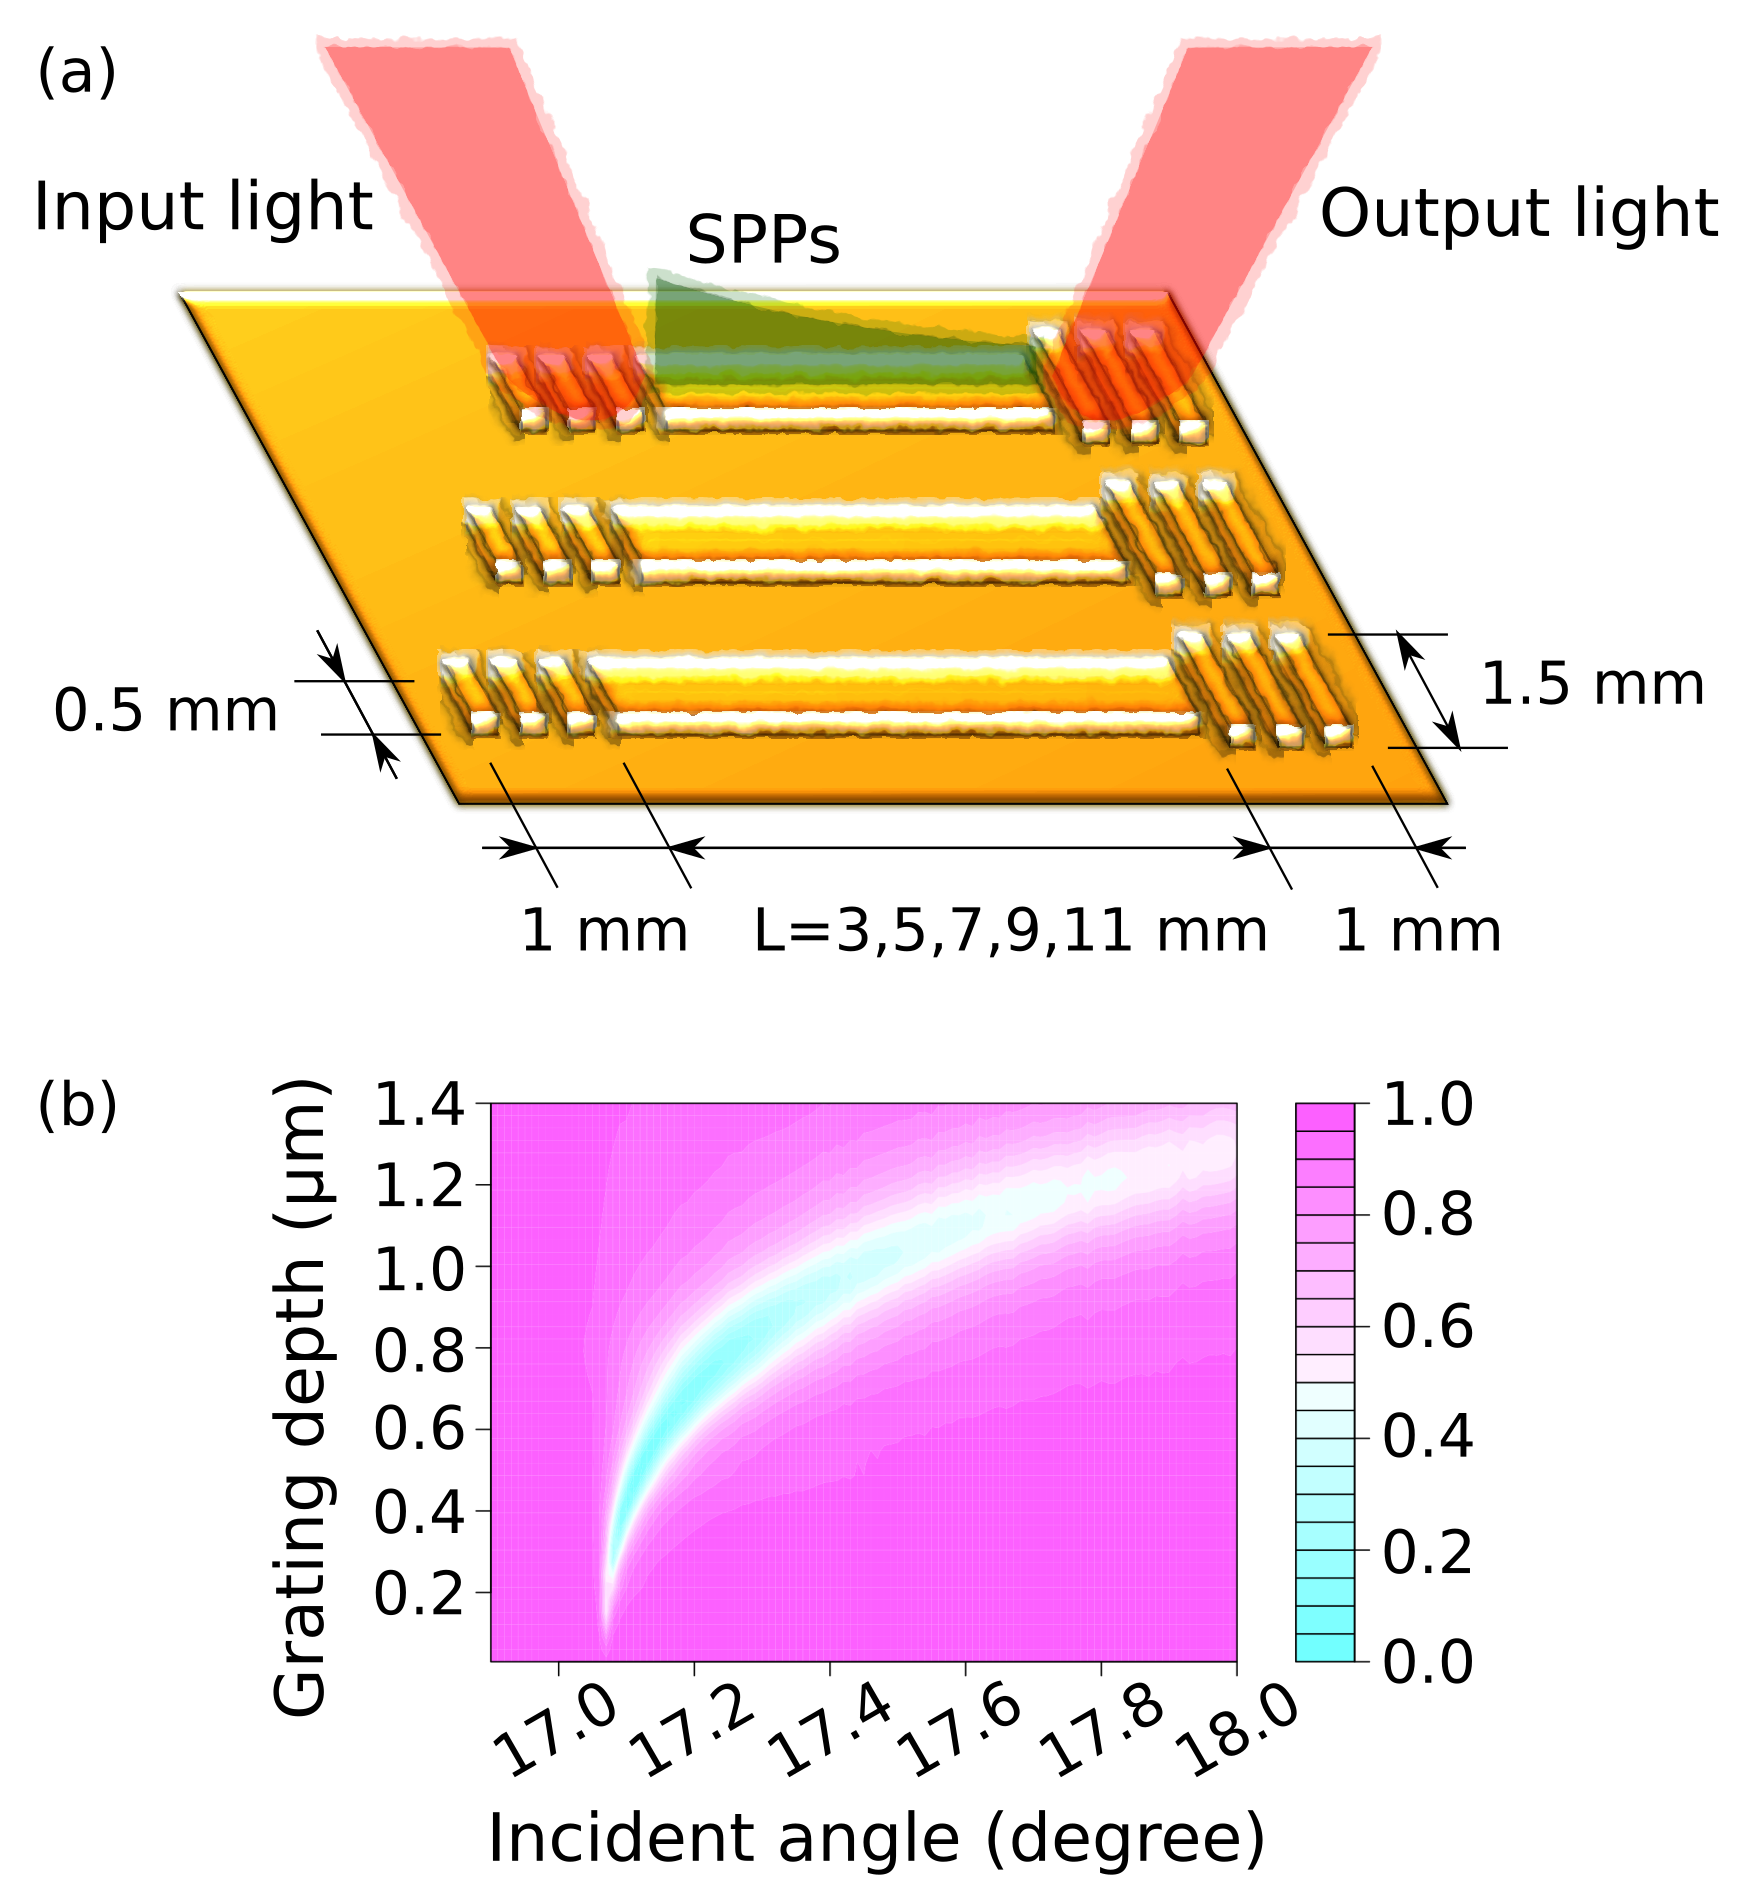
\includegraphics[width=0.8\hsize]{device.eps}
    \caption{(a) Schematic of the SPP waveguide devices. (b) Calculated reflection efficiency of a gold relief grating with a grating pitch of $15\:\mathrm{\mu m}$ and a duty cycle of 0.5, as a function of incident angle and grating depth.}
     \label{fig:device}
\end{figure}

\section{Experiment}
\label{sec:experiment}
Figure \ref{fig:experiment} shows the schematic of our experimental setup. 
A $\mathrm{CO_2}$ laser (L3SL, Access Laser Company) was used as a mid-IR light source generating linearly polarized light at a wavelength of $10.6\:\mathrm{\mu m}$. 
SPP devices were attached to a rotational and 3D-translational stage. 
The p-polarized light (electric field \color{red}lies within \color{black}the plane of incidence) was incident onto the input coupler at the angle that fulfills Eq. \ref{eq:phase-match} where $m=1$, being loosely focused by a spherical mirror with a curvature radius $R$ of $400\:\mathrm{mm}$.  Here the incident light converged with an angle of 1.3 degree to form the beam spot of $0.6\:\mathrm{mm}$ diameter at the sample position. This plane-like wavefront of the incident light and the homogeneous grating coupler should result in a SPP beam with plane-like wavefront. Because the focal depth of the excited SPP beam is about $10\:\mathrm{mm}$, and because the SPPs are confined in the waveguides, we ignored the propagation loss due to diffraction.
The output light was collected by a spherical mirror of $R=150\:\mathrm{mm}$ and a power meter. 
An aperture was placed at the conjugate point of the output coupler to avoid any stray light. 
Time-averaged optical power sent to the input coupler was controlled to be $60\:\mathrm{mW}$ by adjusting the duty ratio of RF power modulation in the $\mathrm{CO_2}$ laser.

In order to modify the morphology of the gold film, the sample containing a series of waveguide devices was annealed twice with a hotplate in argon atmosphere\cite{Nogues}.
In the first annealing process, the sample was heated at $600\:^\circ\mathrm{C}$ for $20\:\mathrm{min}$., and gradually cooled down to room temperature on the hotplate. In the second annealing process, the sample was heated at $700\:^\circ\mathrm{C}$ for $16\:\mathrm{min}$., and cooled down in the same way. The morphology was characterized by AFM (SPA-300, Seiko Instruments Inc.) in tapping mode, and \color{red}by \color{black}SEM/EBSD (JSM-6510LV, JEOL Ltd.) \color{red}with the acceleration voltage of $20\:\mathrm{kV}$.\color{black}

\begin{figure}
    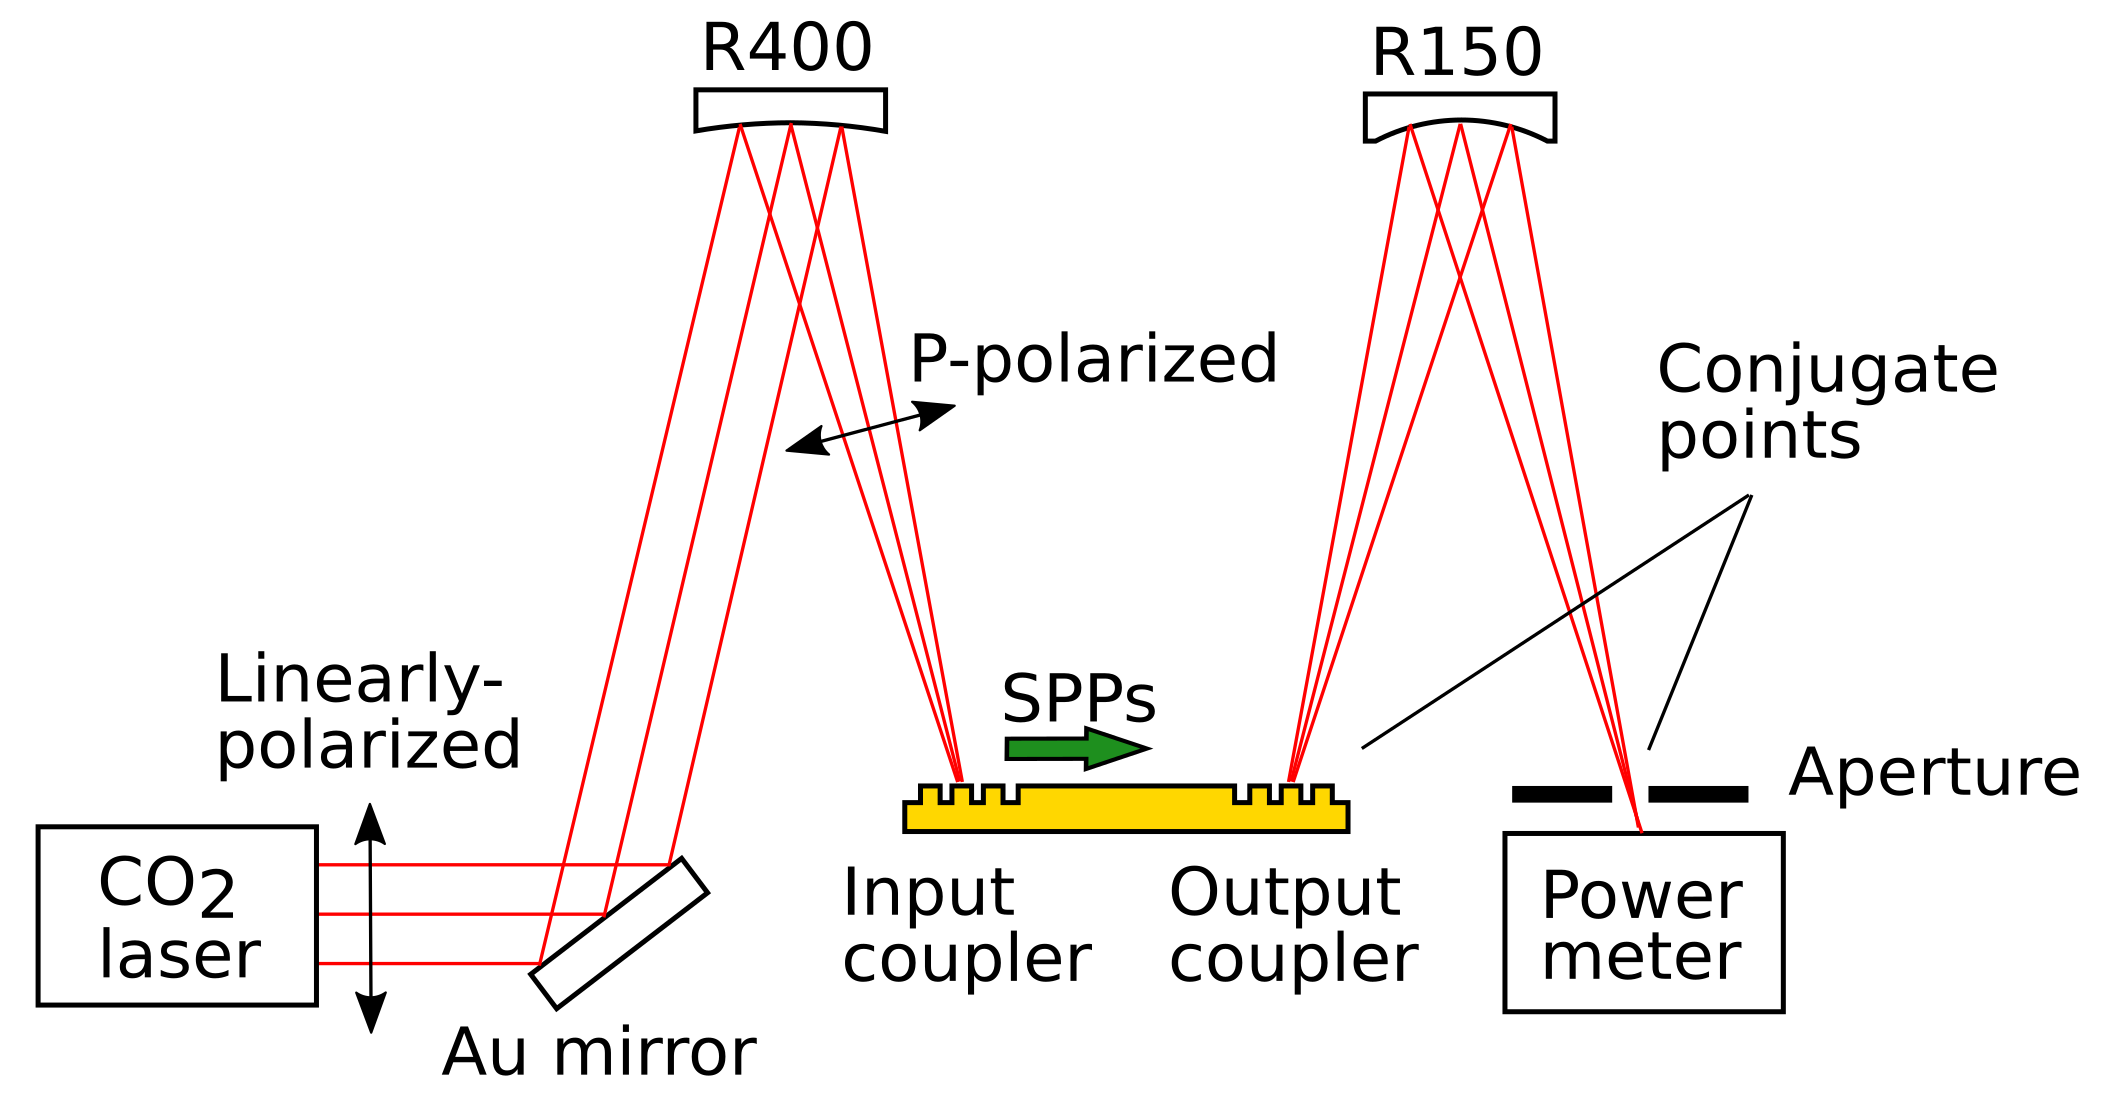
\includegraphics[width=0.85\hsize]{experiment.eps}
    \caption{Schematic of the experimental setup. \color{red}R400 and R150 denote the spherical mirrors with curvature radii of 400 mm and 150 mm, respectively.\color{black}}
     \label{fig:experiment}
\end{figure}

\section{Results}
\label{sec:result}
Figure \ref{fig:propagation_length} shows the measured output power as a function of the waveguide length $L$ for as-grown, once-annealed ($600\:^\circ\mathrm{C}$), and twice-annealed ($600\:^\circ\mathrm{C}$ and $700\:^\circ\mathrm{C}$) samples.
\color{red}Each trace was fitted with the exponential decay function $\exp(-L/L_{\mathrm{SPP}})$ and normalized by the value at $L=0$. Here, \color{black}the propagation length $L_{\mathrm{SPP}}$ was evaluated \color{red}to be \color{black}$9.0\pm0.3\:\mathrm{mm}$, $12.0\pm0.4\:\mathrm{mm}$, and $14.7\pm0.7\:\mathrm{mm}$ for the as-grown, once-annealed, and twice-annealed samples, respectively.
In this way, the SPP propagation length was shown to increase noticeably by the thermal annealing treatment.

\color{red}Figure \ref{fig:morphology} shows an AFM topography \color{black}image (upper panels) of the waveguide surface and \color{red}the corresponding \color{black}cross-sectional height data (lower panels)  for (a) as-grown, (b) once-annealed ($600\:^\circ\mathrm{C}$), and (c) twice-annealed ($600\:^\circ\mathrm{C}$ and $700\:^\circ\mathrm{C}$) samples. Here the sectional surface is indicated as dashed \color{red}lines \color{black}in the topography images.
It is evident from the cross-sectional height data \color{red}that \color{black}surface roughness \color{red}was suppressed by the annealing treatment\color{black}. By calculating root mean squares of deviations in height data, the surface roughness is estimated to be $5.7\:\mathrm{nm}$, $2.8\:\mathrm{nm}$, and $2.2\:\mathrm{nm}$ for the as-grown, once-annealed, and twice-annealed samples, respectively. 
The granular pattern typical for polycrystalline gold was clearly observed for the as-grown sample, as shown in Fig. \ref{fig:morphology}(a). \color{red}Here we \color{black}estimated average diameter of crystallite grains to be $70\pm20\:\mathrm{nm}$ for the as-grown sample, by analyzing the height data with the watershed algorithm\cite{Petr} \color{red}while assuming \color{black}spherical shape for each grain. \color{red}In contrast, \color{black}grain boundaries \color{red}were not identified \color{black}for the annealed samples. Therefore, we \color{red}proceeded to analyze \color{black}the waveguide surface by using SEM and EBSD.

\color{red}Figure \ref{fig:morphology} (d) shows \color{black}a SEM image for the twice-annealed sample. \color{red}It does not identify grain boundaries, nor does the AFM topographic image shown in Fig.\ref{fig:morphology}(c).
Figure \ref{fig:morphology} (e) shows the pattern quality map, \color{black}constructed from the EBSD data, for the same sample and the area as shown in Fig.\ref{fig:morphology}(d). \color{red}Here every point is assigned a brightness based on the EBSD pattern quality for that point. \color{black}Bright \color{red}area \color{black}has high pattern quality (i.e., measured electron diffraction pattern matches well with ideal diffraction pattern of crystalline gold) and indicates crystalline gold. Dark \color{red}area, \color{black}in contrast, has low pattern quality and indicates grain boundary, dislocation, and void. The corresponding inverse pole figure (normal direction) is shown in Fig. \ref{fig:morphology} (f) for reference. \color{red}In this way, the granular pattern is successfully identified by the EBSD measurement. By analyzing the pattern quality data with the watershed algorithm\cite{Petr}, while assuming spherical shape for each grain, we estimated average diameter of crystallite grains to be as large as $2\pm1\:\mathrm{\mu m}$. \color{black}In this way, thermal annealing at $700\:^\circ\mathrm{C}$ or bellow was found to significantly increase the grain size and reduce the surface roughness.

The SPP-light coupling efficiency of the coupler grating \color{red}was \color{black}estimated to be 0.18 \color{red}from \color{black}our experiments. Although optimum incident angle for the maximum coupling efficiency shifted by $\sim0.5^\circ$ upon annealing, the change in the maximum coupling efficiency was not observed. \color{red}Additional \color{black}AFM measurements confirmed that the coupler gratings had ideal rectangular profiles which did not change \color{red}upon annealing.\color{black} 

 \begin{figure}
    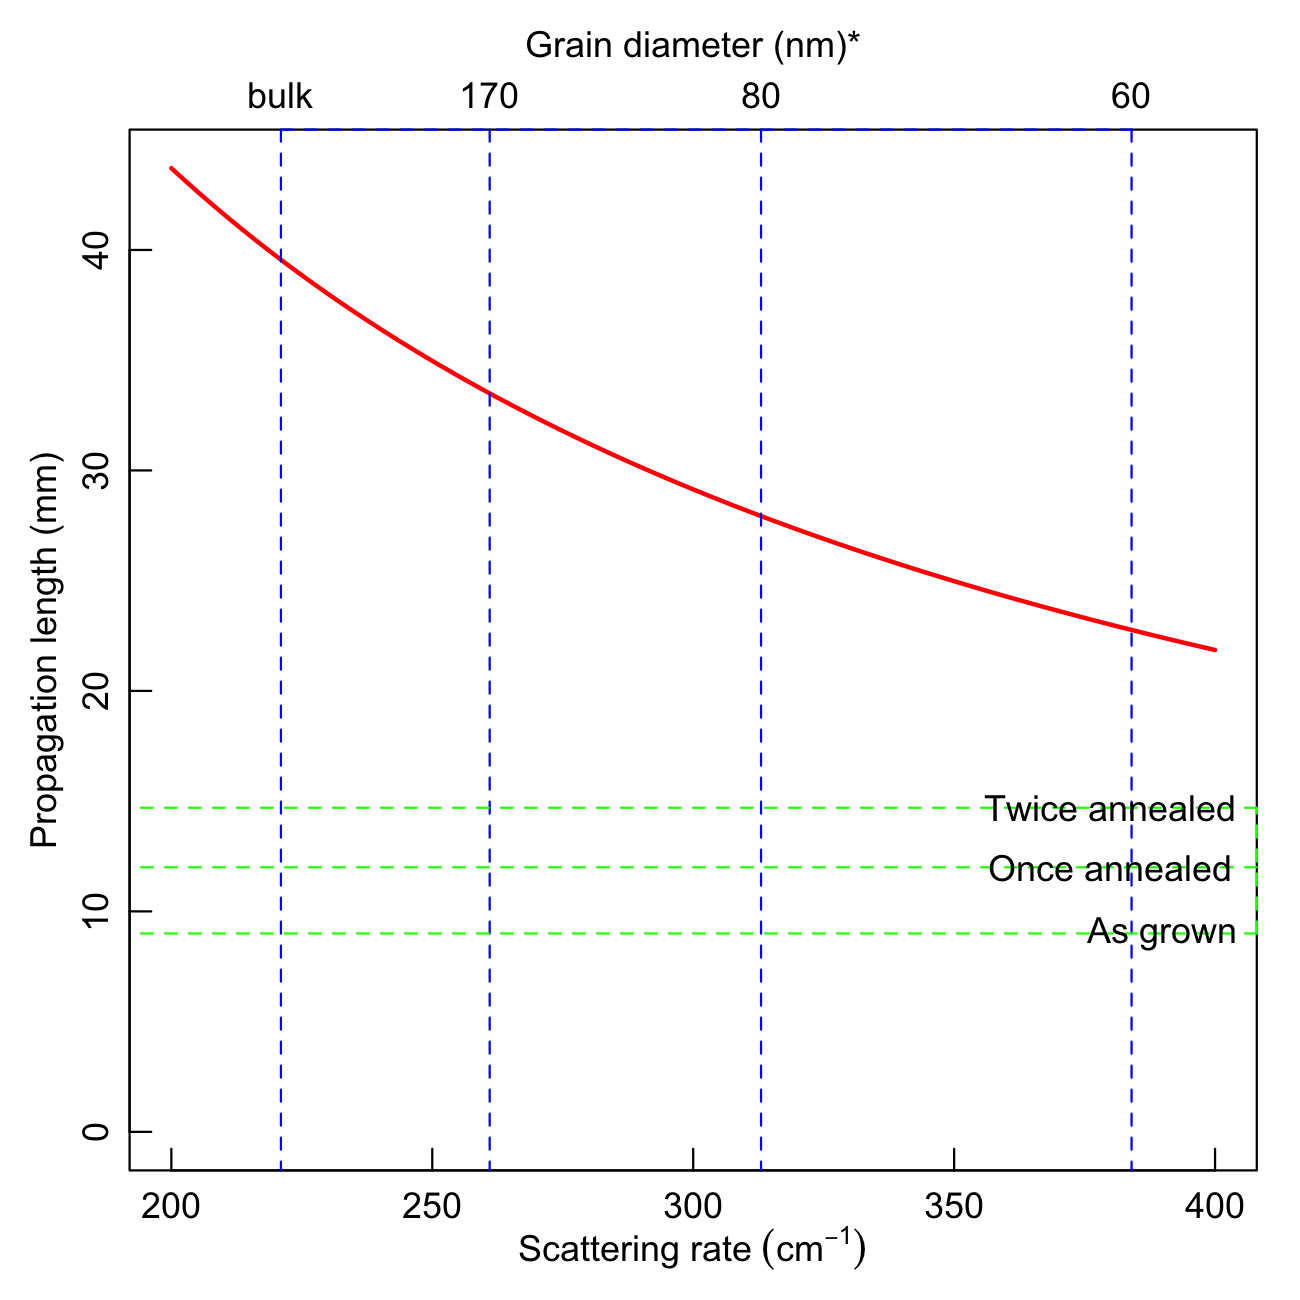
\includegraphics[width=0.85\hsize]{propagation_length.eps}
    \caption{\color{red}Semi-logarithmic plot of \color{black}normalized output power as a function of the SPP waveguide length $L$ for the as-grown(\color{red}squares\color{black}), once-annealed (\color{red}triangles\color{black}), and twice-annealed (\color{red}circles\color{black}) samples. \color{red}Exponential decay curves fitted to these data are also shown as solid lines. \color{black}The propagation length of SPP was evaluated from each trace to be $9.0\pm0.3\:\mathrm{mm}$, $12.0\pm0.4\:\mathrm{mm}$, and $14.7\pm0.7\:\mathrm{mm}$.}
       \label{fig:propagation_length}
\end{figure}

  \begin{figure}
    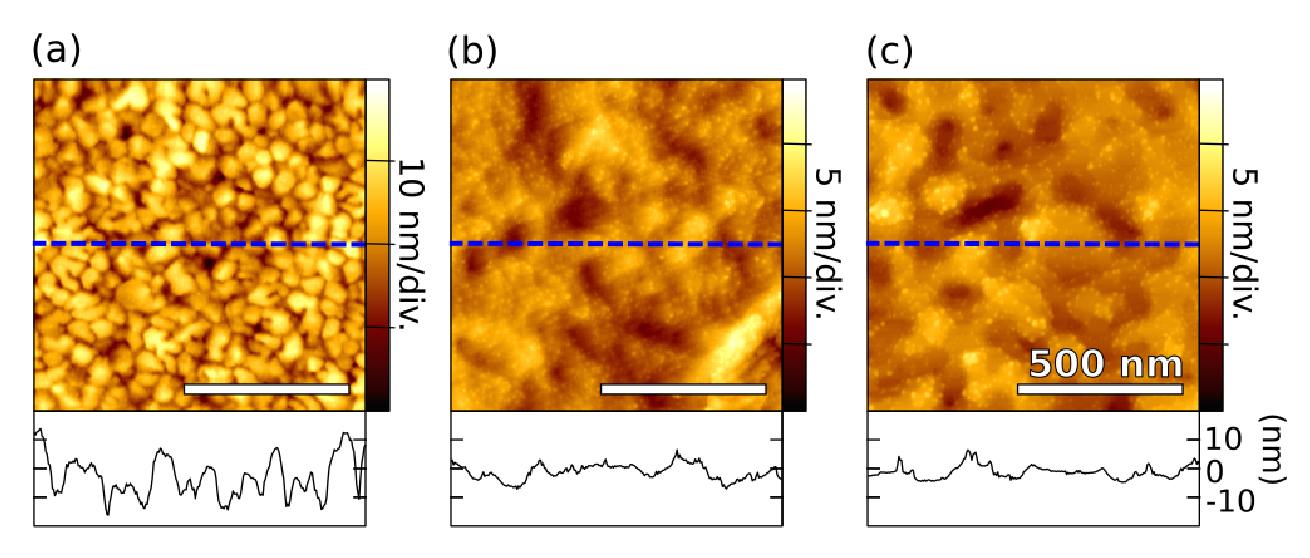
\includegraphics[width=\hsize]{morphology.eps}
        \caption{AFM topography images (upper panels) of the waveguide surface, and the corresponding cross-sectional height data (lower panels) for (a) as-grown, (b) once-annealed ($600\:^\circ\mathrm{C}$), and (c) twice-annealed ($600\:^\circ\mathrm{C}$ and $700\:^\circ\mathrm{C}$) samples. The sectional surface is indicated as dashed lines. \color{red}A SEM image, an EBSD pattern quality map, and an inverse pole figure for the twice-annealed sample are shown in (d), (e), and (f), respectively.\color{black}}
    \label{fig:morphology}
\end{figure}

\section{Discussions}
\label{sec:discussion}
Considering only Ohmic losses, the SPP propagation length $L_{\mathrm{SPP}}$ at a metal/air interface is expressed by the following equation,
\begin{equation}
 L_{\mathrm{SPP}} = \frac{1}{2\:\mathrm{Im} k_{\mathrm{SPP}}},
\label{eq:propagation_length}
 \end{equation}
where $k_{\mathrm{SPP}}=(\lambda/2\pi)\sqrt{\epsilon_g/(\epsilon_g+1)}$ is the complex wavenumber of the SPPs, and $\epsilon_g=\epsilon'_g+i\epsilon''_g$ is the relative dielectric constant of gold. 
By substituting the dielectric constant of polycrystalline gold\cite{Palik} into Eqn. \ref{eq:propagation_length}, \color{red}$L_{\mathrm{SPP}}$ \color{black}is calculated to be $12.3\:\mathrm{mm}$ at a wavelength of $10.6\:\mathrm{\mu m}$.
Our experimentally measured values of  $9.0\pm0.3\:\mathrm{mm}$, $12.0\pm0.4\:\mathrm{mm}$, and $14.7\pm0.7\:\mathrm{mm}$ agree with this theoretical estimation, confirming that mid-IR SPPs at gold/air interface propagates for a distance about or above $>10\:\mathrm{mm}$.

In the following, we will discuss the physics behind the elongation of the SPP propagation length upon thermal annealing, based on our observations of increased grain size (from 70 nm to 2000 nm) and suppressed surface roughness (from 5.7 nm to 2.2 nm). 

Enlargement of the grain size is understood as a resut of the phenomena that smaller crystallite grains preferentially melt upon annealing\cite{Buffat} and re-crystallize into larger particles. 
\color{red} During such phenomena, each crystallite grain can be connected with each other by the necking formation, which would suppress the surface roughness and make unclear the grain boundaries observable with AFM.

SPPs at planer metal/air interface attenuate mainly due to the Ohmic loss  (scattering of free electrons by electrons, phonons, defects, impurities, crystallite grain boundaries, etc.) and partly due to scattering of SPPs by grain boundaries, surface roughness, etc\cite{Kuttge, Lee}. 

Suppressed surface roughness can, in principle, lead to elongated $L_{\mathrm{SPP}}$ by reducing the scattering of SPPs. This contribution, however, would be negligible in our observed elongation of $L_{\mathrm{SPP}}$, since attenuation due to the scattering of SPPs by surface roughness of $<10 \mathrm{mm}$ is estimated to be much smaller than the attenuation, which corresponds to the propagation length on the order of $10 \mathrm{mm}$ at the wavelength of 10.6 $\mathrm{\mu m}$.\cite{Shiba, Kuttge, Mills} 

Trollmann et al.\cite{Trollmann} suggested that surface roughness indicates the existence of empty volume in metal, and that the plasma frequency and the dielectric background increase as the metal volume fraction increases. According to their suggestions, suppression in the surface roughness leads to the increase in the dielectric constant and therefore to the decrease in the SPP propagation length. This hypothesis contradicts with our observations and we discard it as the origin of the elongation of $L_{\mathrm{SPP}}$.

Kuttge et al.\cite{Kuttge} reported that propagation length of SPP at gold/air interface in the visible range is about 5 times larger for the polycrystalline gold film deposited at room temperature (average grain diameter of 80 nm and RMS surface roughness of 1.6 nm) than for that deposited at liquid-nitrogen temperature (average grain diameter of 20nm and RMS surface roughness of 1.3 nm). They attributed the difference in the propagation length to the difference in the Ohmic loss or the scattering rate of electrons. They also needed to take into account the scattering of SPPS at grain boundaries, in order to quantitatively reproduce the measured propagation length.  Trollmann et al.\cite{Trollmann} also assumed that the scattering rate increases with the grain boundary density in explaining (partly) the variation in the dielectric constant. 

Since our observations are in line with these previous reports and therefore it is natural to attribute our observed elongatin of $L_{\mathrm{SPP}}$ to the enlargement of grain size or the reduction of the grain boundary density. The grain boundaries can induce scattering of free electrons\cite{Kuttge, Yang, Trollmann} and scattering of SPPs\cite{Kuttge, Lee}. Simultaneous measurements on dielectric constants may help distinguish the contribution from reduced Ohmic loss from that from reduced scattering of SPPs, both of which origintate from  reduction of grain boundary density.\color{black}

As described above, we have successfully demonstrated that the simple treatment of thermal annealing leads to noticeable elongation of SPP propagation length. It has, however, minor side effect that pinholes may be generated on metal surface. \color{red}In fact, pinholes with diameters on the order of $100 \mathrm{ nm}$ \color{black}appeared with a number density of $0.16\:\mathrm{\mu m}^{-2}$ after the first annealing, and with a number density of $0.44\:\mathrm{\mu m}^{-2}$ after the second annealing. Such pinholes are much smaller than the SPP wavelength but may induce scattering of SPPs. \color{red}Therefore the observed elongation of $L_{\mathrm{SPP}}$ should be the net increase, as a result of competition between contributions from increased grain size and pinholes.\color{black}
	
\section{Conclusions}
\label{sec:conclusion}
We demonstrated that SPPs at gold/air interface propagate for a distance about or above $10\:\mathrm{mm}$ at a wavelength of $10.6\:\mathrm{\mu m}$. The measured propagation length is in good agreement with the value predicted from the dielectric constant of polycrystalline gold. We also successfully demonstrated that the SPP propagation length can be increased by the simple treatment of thermal annealing, accompanied by the increased grain size and the suppressed surface roughness. Quantitative evaluation of the SPP propagation length, correlated with material's morphology, is important in designing plasmonic devices and beneficial for deeper understandings of the mechanism of the losses that underly electric-field enhancement achievable upon SP excitations.

\section*{Acknowledgement}
The authors thank K. Hirakawa and K. Yoshida (Institute of Industrial Science, the University of Tokyo: IIS-UTokyo) for technical supports in thermal evapolation and thermal anneling, T. Takahashi and Y. Shimada (IIS-UTokyo) for technical supports in AFM measurements, M. Maeda, H. Kimura, T. Yoshikawa and T. Narumi (IIS-UTokyo) for technical supports in SEM/EBSD measurements.
%Professor: Masafumi Maeda(64), Kazuhiko Hirakawa(56), Takuji Takahashi(52)
%Assoc. professor: Takeshi Yoshikawa
%Technician: Hisao Kimura, Y. Shimada
%Ph.D. student: Taka Narumi
The sample was fabricated at VLSI Design and Education Center (VDEC), the University of Tokyo. Finantial support by the Japan Society for the Promotion of Science (MEXT KAKENHI 16K13694) is gratefully achnowledged.

\bibliography{Reference}

\end{document}